\chapter{Upravljački program za AD pretvornik ADS131M08}

    \section{Opis rada sklopa ADS131M08}
        ADS131M08 je 24-bitni, 8 kanalni delta-sigma analogno-digitalni pretvornik \engl{Analog to Digital Converter, ADC} proizvođača Texas Instruments \cite{ads131m08_datasheet}. Za komunikaciju s mikrokontrolerom koristi SPI sučelje. Svih 8 kanala uzorkuje se istovremeno, a za svaki kanal moguće je postaviti programibilno pojačanje od 1 do 128. Frekvencija uzorkovanja također je programibilna i može iznositi do 32 tisuće uzoraka u sekundi. Slika \ref{fig:adt7301_blok_dijagram} prikazuje blok dijagram sklopa.

        \begin{figure}[htb]
            \centering
            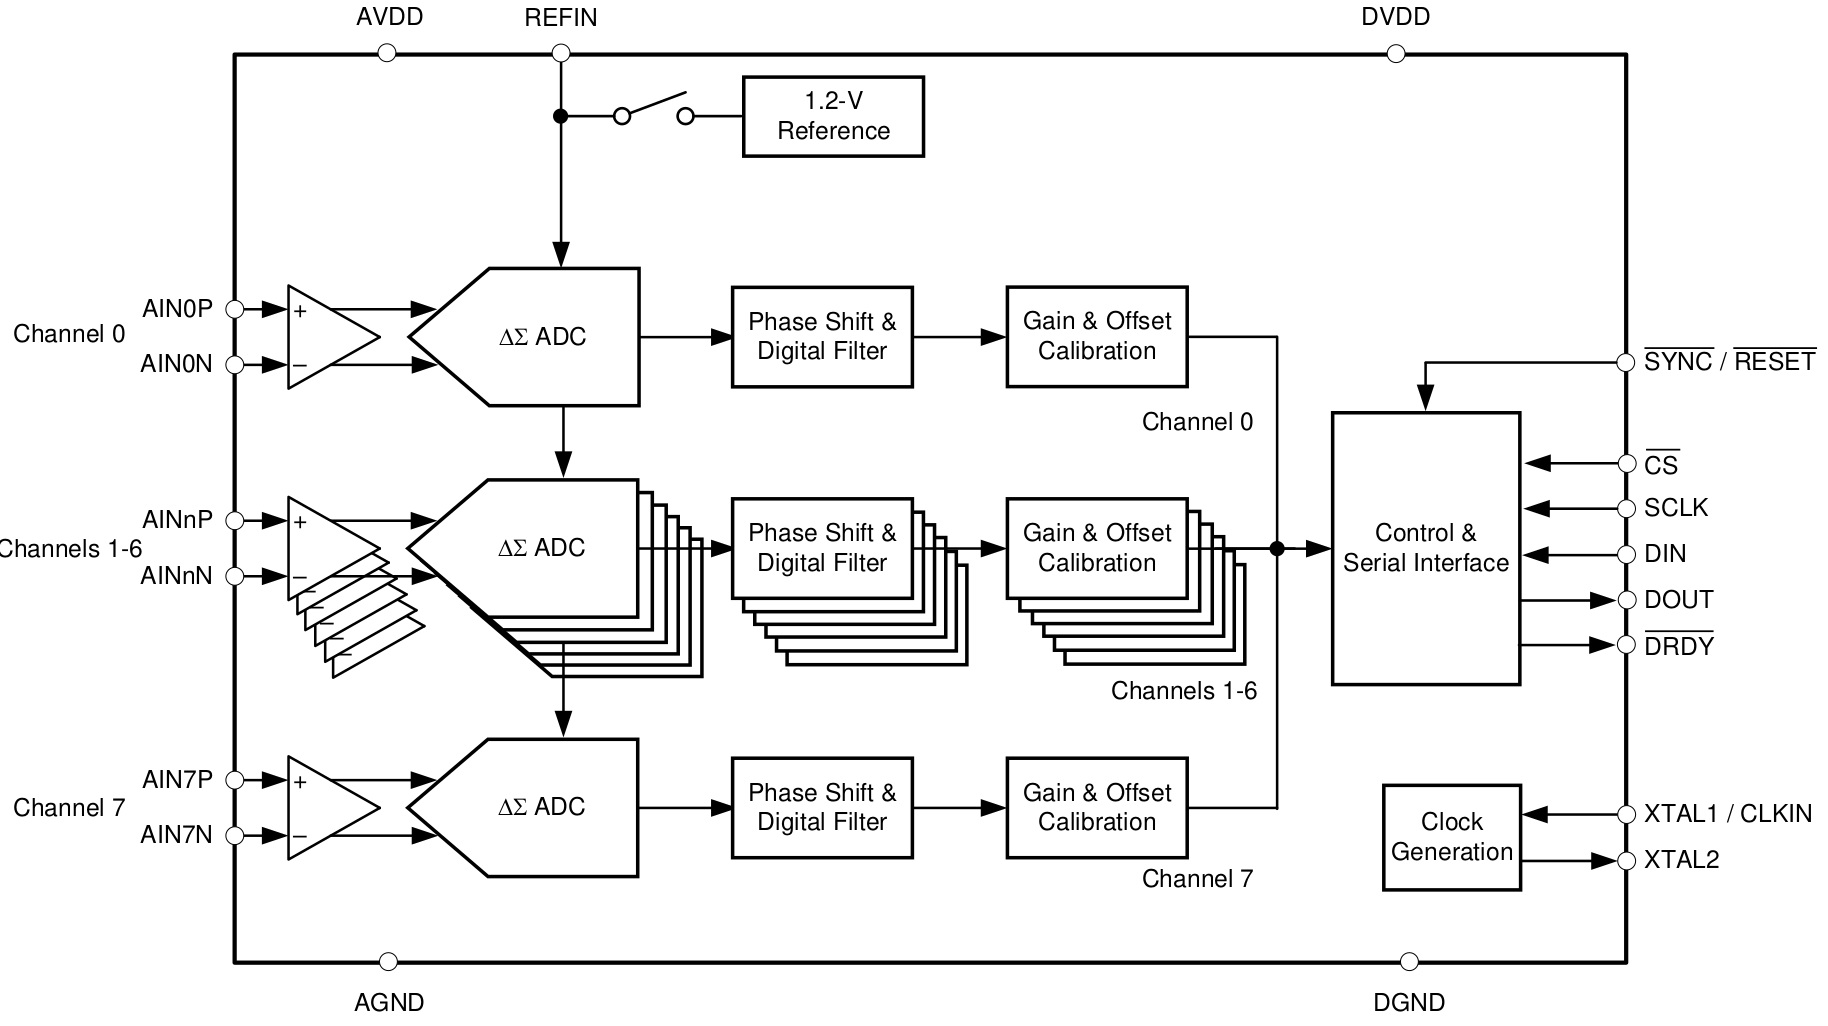
\includegraphics[width=\textwidth]{slike/ads131m08_blok_dijagram.png}
            \caption{Blok dijagram sklopa ADS131M08 \cite{ads131m08_datasheet}}
            \label{fig:ads131m08_blok_dijagram}
        \end{figure}

        Sklop zahtijeva odvojeno napajanje digitalnog i analognog dijela. Analogno napajanje može biti u rasponu 2.7 - 3.6 V, a digitalno napajanje treba biti 1.8 V ili 3.3 V. Referentni napon se može dovesti na vanjski priključak, ili se može koristiti unutarnji izvor referentnog napona iznosa 1.2 V. Signal takta može se generirati unutar sklopa ili može biti doveden na vanjski priključak. 

    \section{SPI sučelje}
        SPI sučelje sklopa ADS131M08 koristi postavke CPOL = 0 i CPHA = 1, što znači da niska logička razina odgovara neaktivnom stanju takta i da se podatak čita na drugi brid takta (padajući). Za komunikaciju se koriste standardni SPI priključci (SCLK, MOSI, MISO i \textoverline{CS}) i dva dodatna priključka: \textoverline{DRDY} (\textit{Data Ready}) i \textoverline{SYNC/RESET}.
        
        \textoverline{DRDY} priključak postaje aktivan u trenutku kada je sklop spreman poslati rezultate konverzije. Aktiviranje priključka može se iskoristiti za okidanje prekida na mikrokontroleru, što omogućuje pravovremeno čitanje. Posebnu pažnju treba obratiti kada se podaci čitaju prvi put nakon uključenja ili kada je prošlo dulje vrijeme od zadnjeg čitanja. Naime, ADC ima unutarnji međuspremnik u kojem se spremaju rezultati konverzije ako nisu pročitani. Međuspremnik ima dovoljno kapaciteta za spremanje posljednje dvije konverzije. Kada je međuspremnik pun, ponašanje priključka \textoverline{DRDY} neće biti dosljedno. Proizvođač zato preporuča dva načina za sinkronizaciju: prvi je pročitati dva uzorka zaredom bez čekanja aktivacije \textoverline{DRDY} priključka i tako isprazniti međuspremnik \cite[str.~40]{ads131m08_datasheet}. Drugi način sinkronizacije je postavljanje pravokutnog impulsa trajanja duljeg od jednog perioda signala takta ADC-a, ali kraćeg od 2048 perioda na priključak \textoverline{SYNC/RESET} \cite[str.~40, 46]{ads131m08_datasheet}.

        Podaci se prenose preko SPI sučelja u takozvanim okvirima. Svaki okvir sastoji se od 10 riječi (ili manje, ako su neki kanali onemogućeni). Duljina riječi može se postaviti na 16, 24 ili 32 bita, a pretpostavljena duljina je 24 bita. Sučelje radi u \textit{Full-Duplex} načinu rada. Vremenski dijagram jednog okvira prikazan je na slici \ref{fig:ads131m08_spi_vremenski_dijagram}.

        \begin{figure}[htb]
            \centering
            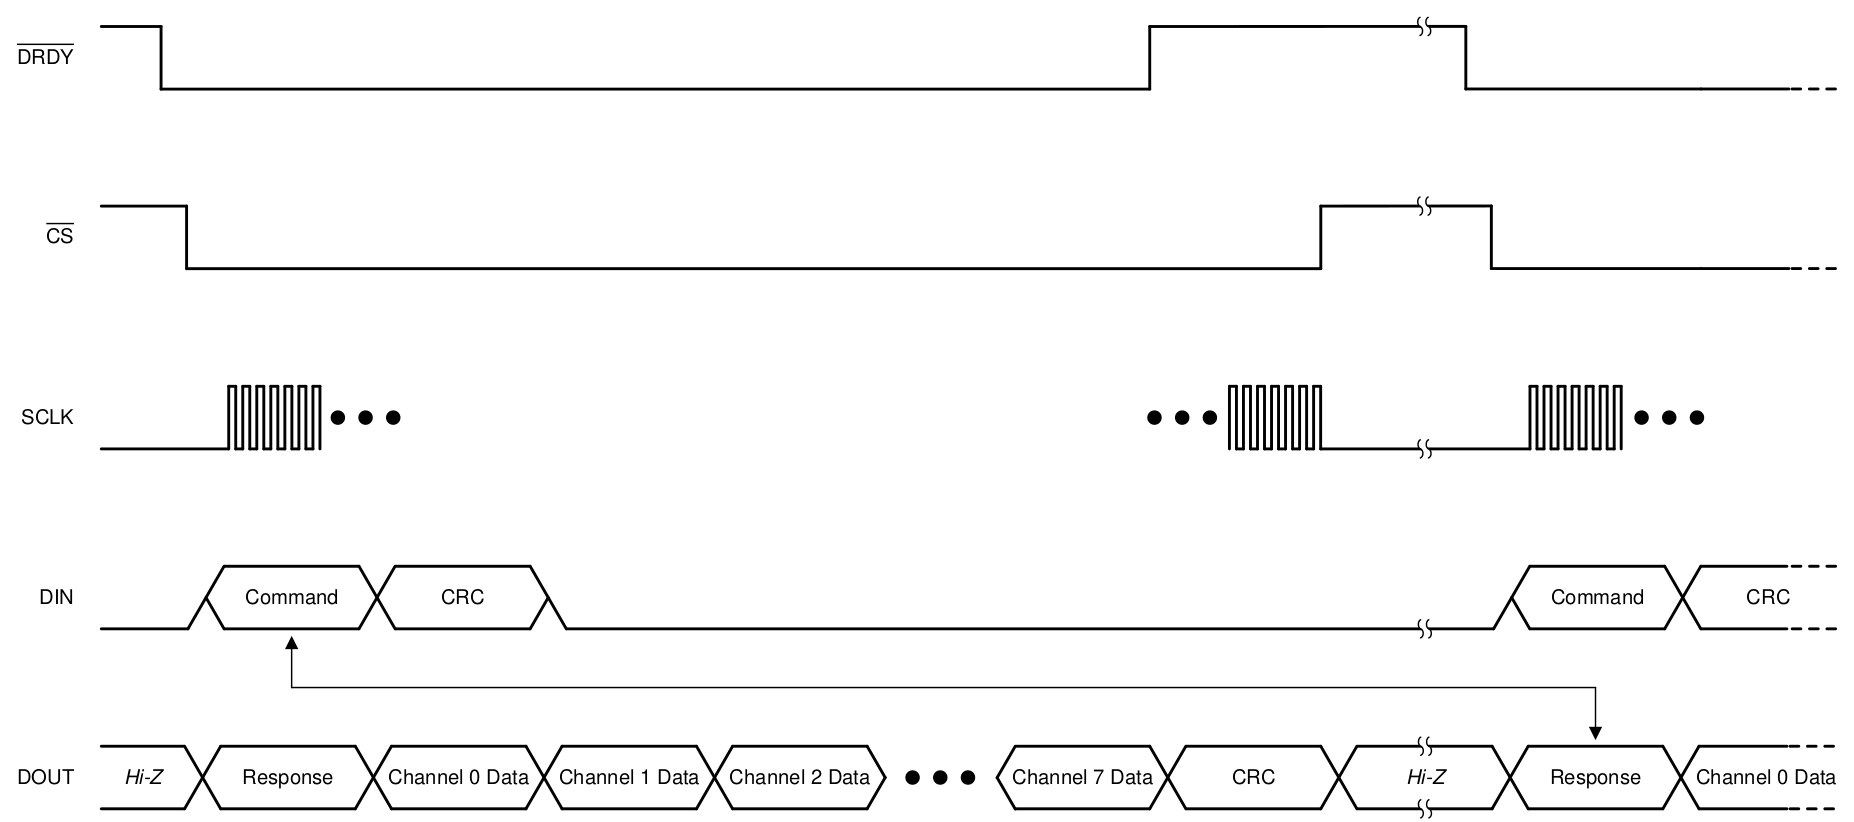
\includegraphics[width=\textwidth]{slike/ads131m08_spi_vremenski_dijagram.png}
            \caption{Vremenski dijagram SPI komunikacije. Strelica označava naredbu i pripadajući odgovor. \cite{ads131m08_datasheet}}
            \label{fig:ads131m08_spi_vremenski_dijagram}
        \end{figure}

        Prva riječ okvira na liniji MOSI (na slici označeno DIN) jest naredba koju \textit{master} uređaj šalje ADC-u. Najčešće korištena naredba je \textit{Null} naredba, čiji je instrukcijski kod 0x0000. Kada primi tu naredbu, ADC neće obaviti nikakvu operaciju, već će samo poslati rezultate konverzije. Neke druge naredbe su RREG (čitanje registra), WREG (upis u registar) i RESET. Druga riječ okvira je CRC (\textit{Cyclic Redundancy Check}) zaštitni kod poruke (ili riječ bitova u niskoj razini ako je CRC onemogućen), nakon čega slijedi 8 riječi s bitovima u niskoj logičkoj razini.

        Prva riječ okvira na liniji MISO (na slici označeno DOUT) jest odgovor na naredbu u prethodnom okviru. Ako je naredba bila \textit{Null}, tada je odgovor ispis sadržaja registra stanja ADC-a. U slučaju neke druge naredbe odgovor se može sastojati i od više riječi, na primjer ako se radi o ispisu sadržaja nekoliko registara. Nakon odgovora slijedi 8 riječi, po jedna za svaki kanal, koje sadrže rezultate AD pretvorbe. Moguće je onemogućiti neke kanale korištenjem naredbe WREG, u tom će slučaju riječ koja odgovara tom kanalu biti izostavljena. Posljednja riječ u okviru je CRC zaštitni kod poruke.
        